\chapter{DPS Annotation Framework}

\section{Motivation for DPS}

A central methodological challenge in this project is how to convert mobile application screenshots into analyzable evidence of dark pattern exposure. Prior research on dark patterns has developed conceptually rich taxonomies that distinguish many types of deceptive or manipulative interface designs, including nagging, obstruction, sneaking, interface interference, forced action, scarcity messages, social proof, hidden costs, preselection, and other forms of choice manipulation \cite{gray2018darkpatterns,mathur2019darkpatterns,mathur2021whatmakesdark}. These taxonomies are valuable because they reveal the diversity of dark pattern mechanisms and provide a theoretical vocabulary for discussing how interfaces may influence user decisions. However, their richness also creates a practical difficulty for screenshot-level annotation. When an annotator observes a single screen in a mobile app, it is often difficult to decide which fine-grained category best describes the interface, especially when several mechanisms appear simultaneously.

For example, a membership popup may visually emphasize an ``Activate Now'' button, hide the close icon, and use wording that suggests the offer is urgent. A fine-grained taxonomy might classify these elements separately as visual interference, obstruction, urgency, or misdirection. In practice, however, requiring annotators to choose from many overlapping labels can reduce consistency and make large-scale annotation difficult. Since this project collects 1,440 interaction records and assigns seven labels to each record, producing 10,080 DPS labels in total, the annotation scheme must be compact, reproducible, and easy to apply across different apps and profiles.

The DPS framework is designed to address this need. Instead of reproducing every category from previous taxonomies, it abstracts common dark pattern mechanisms into seven dimensions that can be applied at the screenshot level. This abstraction does not replace prior taxonomies; rather, it operationalizes them for the specific purpose of profile-aware auditing. The goal is not to identify every possible subtype of dark pattern, but to measure whether different controlled user profiles are exposed to different kinds of manipulative interface mechanisms during mobile app interaction. In this sense, DPS serves as a bridge between qualitative dark pattern concepts and quantitative exposure analysis.

This compact representation is also necessary because the project studies exposure as a distributional outcome. Each screenshot is treated as one observation generated under a particular app, profile, and interaction step. To compare exposure across profiles, the project needs a consistent vector representation that can be averaged, compared, and statistically tested. The DPS vector therefore provides the basis for estimating profile-conditioned exposure, computing pairwise exposure differences, drawing heatmaps, plotting running mean convergence curves, and conducting permutation-based validation.

\begin{figure}[htbp]
    \centering
    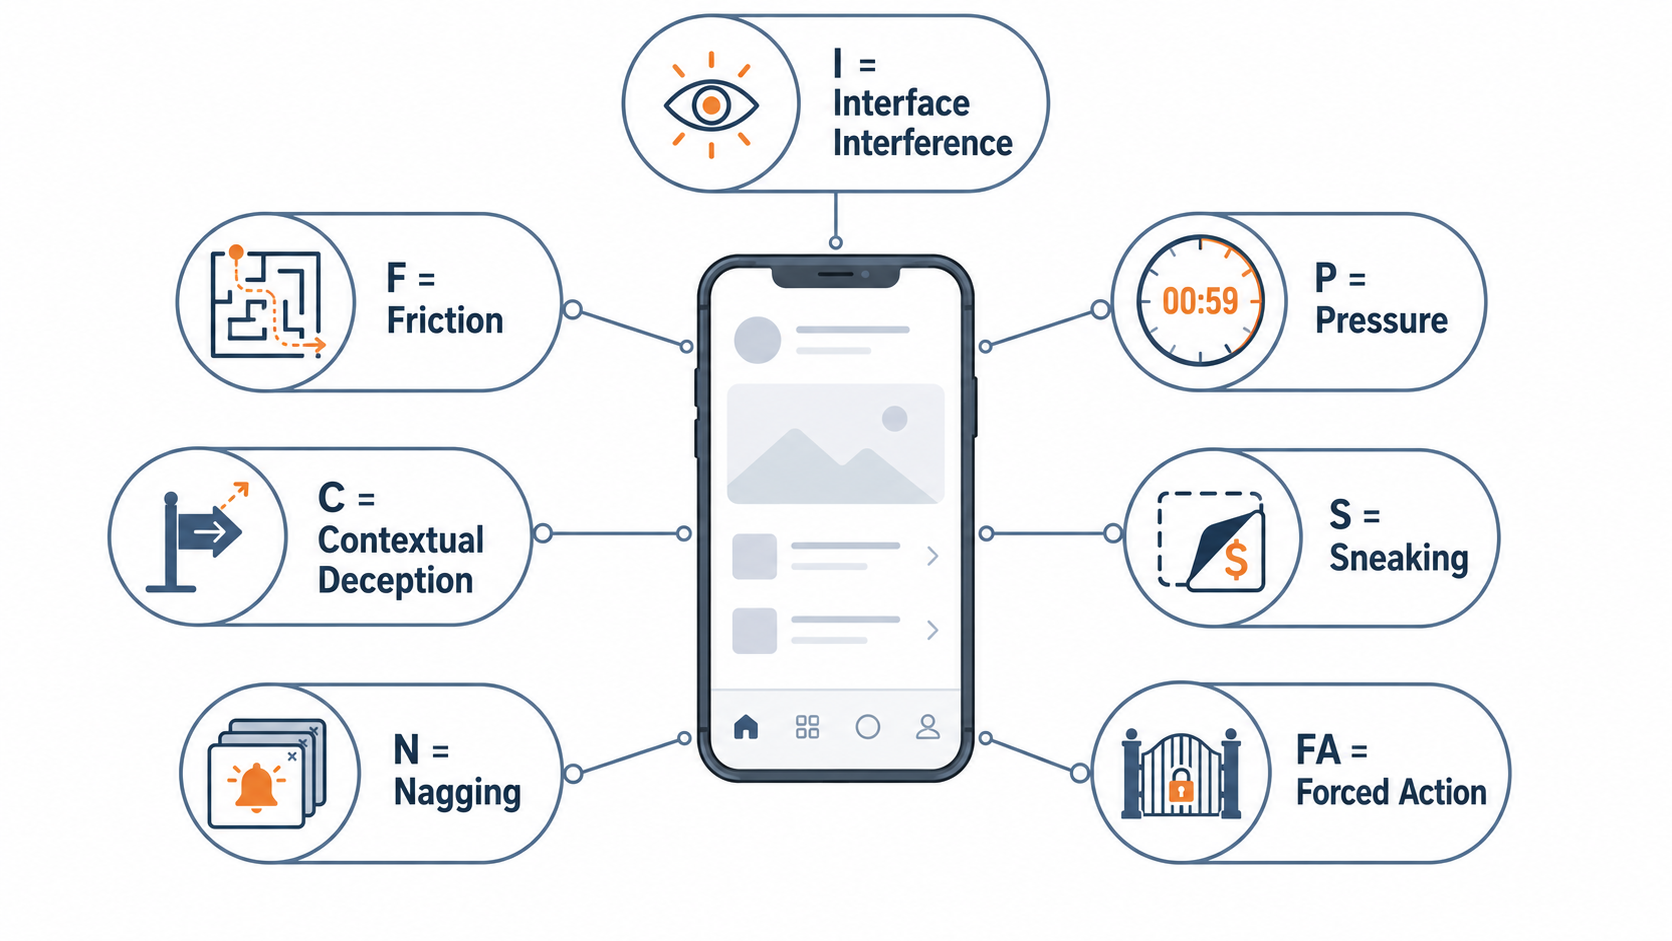
\includegraphics[width=0.95\linewidth]{figures/pictures/seven-dimensional_DPS_vector.png}
    \caption{Seven-Dimensional DPS Vector}
    \label{fig:seven-dimensional-dps-vector}
\end{figure}

\section{DPS Vector Definition}

The project represents dark pattern exposure using a seven-dimensional vector called DPS, defined as follows:

\[
\mathrm{DPS} = [I, F, P, C, S, N, FA],
\]

where \(I\) denotes Interface Interference, \(F\) denotes Friction, \(P\) denotes Pressure, \(C\) denotes Contextual Deception, \(S\) denotes Sneaking, \(N\) denotes Nagging, and \(FA\) denotes Forced Action. Each screenshot collected during the interaction trajectory is converted into one DPS vector. The vector records whether the screen contains observable evidence of each dimension.

This vector-based representation has three advantages.

\begin{itemize}
    \item It allows different dark pattern mechanisms to co-exist in the same screenshot. A screen may contain both pressure and interface interference, or both forced action and nagging.
    \item It avoids forcing annotators to choose a single dominant category when multiple mechanisms are present.
    \item It supports quantitative comparison across profiles. Once every screenshot is represented as a vector, exposure can be aggregated by app, profile, step, or DPS dimension.
\end{itemize}

In the current implementation, each dimension is annotated as a binary label. For a given screenshot, the value of a dimension is 1 if the corresponding mechanism is present and 0 if it is absent. For example, a screenshot with a countdown timer and a visually emphasized purchase button might be annotated as having pressure and interface interference. A screenshot that requires the user to log in before browsing may be annotated as forced action. The following subsections define each DPS dimension and provide practical annotation guidance.

\section{Interface Interference}

Interface Interference refers to visual or layout manipulation that changes how users perceive available options. It occurs when the interface does not present choices in a neutral or balanced way, but instead visually steers attention toward the platform-preferred option. This dimension is closely related to earlier discussions of manipulative choice architecture and interface interference in dark pattern research \cite{gray2018darkpatterns,mathur2021whatmakesdark}.

A typical example is a popup in which the accept button is large, colorful, and centrally placed, while the reject or close option is tiny, gray, or placed in a corner. Another example is a consent or membership interface where the beneficial option for the platform is highlighted with strong contrast, while the user-protective option is visually minimized. Interface interference may also appear when important information is displayed in small gray text, when the close icon is hidden or visually blended into the background, or when misleading color contrast makes one option appear safer, more natural, or more recommended than another.

The key annotation principle is that Interface Interference should be marked when the visual structure of the screen appears to bias perception of choices. It is not necessary to prove that the user was actually deceived. The annotator only needs to judge whether the layout, color, size, placement, or visibility of interface elements gives unequal perceptual weight to different options. For instance, if a shopping app shows a large orange ``Buy Now'' button and places ``Continue Browsing'' in small gray text at the bottom, the screenshot may be labeled as Interface Interference. If all options are presented with comparable visibility and emphasis, this dimension should normally be marked as absent.

\section{Friction}

Friction refers to additional effort imposed on certain user choices, especially rejecting, canceling, opting out, or exiting. It becomes problematic when the effort is asymmetric: one path is easy, immediate, and visually obvious, while the alternative path requires more steps, repeated confirmation, or hidden navigation. This dimension captures the practical difficulty of exercising a choice, rather than the visual appearance of the choice alone.

For example, canceling a membership may require several screens, while renewing the same membership requires only one tap. Rejecting a promotion may require opening a secondary menu, while accepting it is available on the first screen. An exit path may be hidden behind a small icon or placed outside the main interaction flow. In some cases, the user may be redirected repeatedly before refusal is finally allowed. These patterns do not necessarily deceive the user about what is happening, but they make the undesired choice more burdensome.

The annotation should focus on observable interaction burden. If the screenshot clearly indicates that continuing, accepting, or purchasing is easier than refusing, canceling, or exiting, Friction should be marked as present. However, not every multi-step process should be labeled as friction. Some tasks naturally require multiple steps for security or technical reasons, such as confirming a payment or verifying identity. Friction becomes relevant to DPS when the burden appears selectively attached to the user-protective or platform-dispreferred option. Therefore, annotators should ask whether the interface imposes extra effort asymmetrically, rather than simply whether the screen is complex.

\section{Pressure}

Pressure refers to temporal, emotional, scarcity-based, or social cues that push users toward quick decisions. It captures interface elements that create urgency or anxiety, encouraging users to act before they have fully evaluated the choice. This dimension is associated with dark pattern categories such as urgency, scarcity, social proof, and confirmshaming discussed in previous studies of online shopping and deceptive interface design \cite{mathur2019darkpatterns}.

Examples include countdown timers, limited-time offers, labels such as ``only 2 left,'' statements such as ``many people are viewing this,'' and fear-of-missing-out messages. A discount page may show a timer suggesting that the price will disappear soon. A food-delivery app may display a promotion with wording such as ``Order now before the coupon expires.'' A shopping app may state that an item is selling fast or that other users have recently purchased it. These messages may be legitimate in some cases, but from an annotation perspective they still count as pressure when they are used to accelerate the user's decision.

Annotators should mark Pressure as present when the screenshot contains explicit urgency, scarcity, emotional appeal, or social comparison cues. The label does not require determining whether the claim is true or false. For example, the project does not need to verify whether only two items are actually left in stock. The relevant question is whether the interface uses such a cue to influence the user's decision-making context. If a promotion simply states a price or discount without urgency or emotional framing, Pressure should generally be marked as absent.

\section{Contextual Deception}

Contextual Deception refers to a mismatch between what the user reasonably expects in the current interface context and what an action actually does. In this project, \(C\) specifically means Contextual Deception, not merely confusion. A confusing interface may be poorly designed, but it should be labeled as Contextual Deception only when the screen creates a misleading relationship between the apparent meaning of an action and its actual consequence.

For example, a button may appear to close a popup but instead open a subscription page. Ambiguous wording may hide the actual consequence of clicking, such as making a payment, joining a membership program, or enabling automatic renewal. A button placed near a browsing element may cause accidental transition to checkout. A user who intends to view product details may unexpectedly be redirected to a payment or membership interface. In these cases, the deception is contextual because the meaning of the action depends on the surrounding interface situation.

The annotation should consider the user's likely expectation at that moment. If a close-like icon, back-like button, or neutral browsing action leads to a consequence that is inconsistent with its apparent function, Contextual Deception should be marked as present. By contrast, if the consequence is clearly stated and visually aligned with the action, this dimension should be absent even if the user might dislike the result. This distinction is important because the DPS framework aims to capture deceptive context-action mismatches, not all forms of inconvenience or dissatisfaction.

\section{Sneaking}

Sneaking refers to hiding, delaying, or quietly adding information that affects user decisions. It often appears near checkout, subscription, or membership interfaces, where additional costs or commitments may be introduced without being made salient. This dimension is connected to prior dark pattern categories such as hidden costs, sneak into basket, preselection, and default add-ons \cite{gray2018darkpatterns,mathur2019darkpatterns}.

Examples include hidden fees that are revealed only at the final step, preselected paid add-ons, default inclusion of a subscription, or an extra service added near checkout. A shopping app may automatically select shipping insurance. A food-delivery app may add a paid membership trial by default. A travel or ticketing app may reveal service fees only after the user has already invested effort in the booking process. These mechanisms affect decision-making because the user may proceed under an incomplete understanding of cost or commitment.

Annotators should mark Sneaking as present when the screenshot shows evidence that a cost, service, subscription, or commitment has been added, hidden, delayed, or preselected in a way that may not be immediately expected. If the additional item is clearly optional, not preselected, and equally visible, Sneaking should normally be absent. The key question is whether the interface quietly changes the transaction or decision context in favor of the platform.

\section{Nagging}

Nagging refers to repeated interruptions after users dismiss or ignore a request. Unlike Pressure, which focuses on urgency or emotional influence, Nagging focuses on repetition and interruption. It occurs when the application repeatedly asks the user to perform an action, even after the user has already declined or ignored similar prompts.

Common examples include repeated membership popups, repeated notification permission requests, repeated login prompts, and repeated promotional interruptions. A user may close a membership discount popup, only to see a similar popup again after scrolling or opening another page. A mobile app may repeatedly request notification permission each time the user enters the home screen. A browsing session may be interrupted by login prompts even when login is not necessary for the immediate task.

In annotation practice, Nagging is easiest to identify when interaction history is available. A single screenshot may show a popup, but the nagging label depends on whether similar interruptions have appeared repeatedly during the trajectory. Therefore, annotators should use the current screenshot together with the previous interaction records when judging this dimension. If the same type of request appears repeatedly after dismissal or avoidance, Nagging should be marked as present. If a request appears only once and is relevant to the current task, it should generally not be labeled as nagging.

\section{Forced Action}

Forced Action means that the user must perform an additional action before accessing the intended function. It captures situations where the app blocks the user's original goal unless the user completes a platform-required step. This dimension is derived from prior dark pattern taxonomies that identify forced action as a mechanism for extracting registration, consent, permissions, or other commitments from users \cite{gray2018darkpatterns}.

Examples include requiring login before browsing, requiring notification permission before entering the app, requiring phone-number binding before using a feature, requiring acceptance of unrelated terms, or requiring the user to complete an extra task before continuing. Forced Action is especially relevant in mobile apps because many apps combine browsing, shopping, payment, social features, and account systems in a single interface. As a result, users may encounter blocking screens that require them to provide data, accept permissions, or join programs before reaching the intended function.

Annotators should mark Forced Action as present when access to the user's apparent goal is blocked until an additional action is completed. The label should not be used when the requested action is strictly necessary for the function. For example, payment naturally requires payment confirmation, and account recovery naturally requires identity verification. However, if the user simply wants to browse products and is required to log in, bind a phone number, or enable notifications, Forced Action should be marked as present. In the project findings, some app categories, such as food-delivery apps, show consistently high forced-action exposure, suggesting that this dimension is important for understanding how access control and commercial goals interact in mobile interface design.

\section{Annotation Scale}

In the current version of the DPS framework, each dimension is annotated using a binary scale:

\[
d_i \in \{0, 1\},
\]

where \(d_i = 1\) means that the corresponding DPS dimension is present in the screenshot, and \(d_i = 0\) means that it is absent. A complete DPS vector therefore consists of seven binary values. For example, a screenshot may be represented as:

\[
[1, 0, 1, 0, 0, 0, 0],
\]

which indicates that Interface Interference and Pressure are present, while Friction, Contextual Deception, Sneaking, Nagging, and Forced Action are absent.

The binary scale is chosen for consistency and feasibility. Since the experiment involves 16 apps, 3 profiles, and 30 interaction steps per profile-app pair, the annotation workload is already substantial. A binary scheme reduces ambiguity and allows annotators to focus on whether a mechanism is observable. It also supports straightforward aggregation. For each profile \(A\), the project can estimate the expected exposure \(E(D \mid A)\) by averaging DPS labels across records. Pairwise differences between profiles can then be computed as \(\Delta(A_i, A_j)\), and statistical validation can be conducted using permutation tests, q-values, L1 distance, and Cramér's V.

Future work could extend the binary scale to ordinal scores such as 0, 1, and 2, where 0 indicates absence, 1 indicates weak or moderate presence, and 2 indicates strong presence. Such an extension would allow more nuanced measurement of severity. For example, a small countdown label and a full-screen urgent warning might both be labeled as Pressure under the binary scale, while an ordinal scale could distinguish their intensity. However, ordinal scoring also requires stronger annotation guidelines and reliability checks. For the present course project, the binary scale provides a practical balance between expressiveness and consistency.

\begin{figure}[htbp]
    \centering
    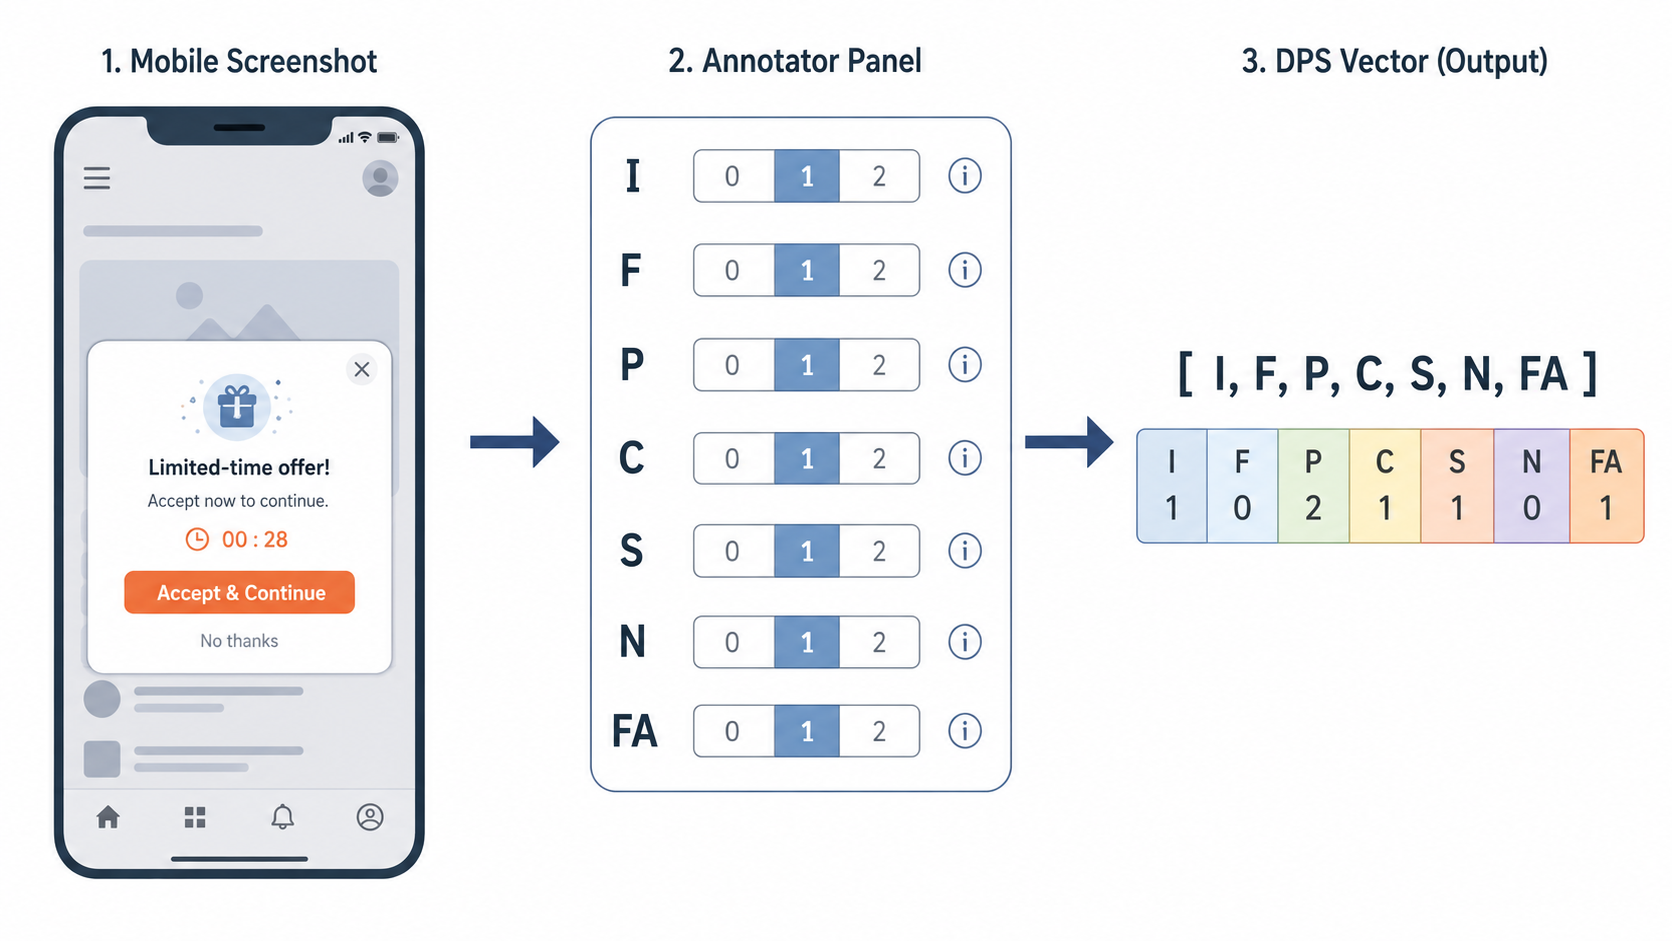
\includegraphics[width=0.95\linewidth]{figures/pictures/from_screenshot_to_DPS_label.png}
    \caption{From Screenshot to DPS Label}
    \label{fig:from-screenshot-to-dps-label}
\end{figure}

\section{Annotation Examples}

Consider a membership popup with a large ``Activate Now'' button and a small close icon in the upper corner. A possible DPS vector is:

\[
[1, 0, 0, 0, 0, 0, 0].
\]

Interface Interference is marked as present because the platform-preferred action is visually emphasized while the exit option is minimized. If the popup appears repeatedly after dismissal, Nagging may also be marked as present, resulting in \([1, 0, 0, 0, 0, 1, 0]\). If the user cannot continue using the app without activating or logging in, Forced Action may also be present. This example shows why DPS annotation should consider both the screenshot and the interaction context.

A second example is a discount page with a countdown timer and wording such as ``limited quantity'' or ``only 2 left.'' A possible vector is:

\[
[0, 0, 1, 0, 0, 0, 0].
\]

Pressure is marked as present because the interface uses temporal urgency and scarcity cues to encourage quick decision-making. If the page also uses a large purchase button and a visually weak refusal option, Interface Interference may be added, producing \([1, 0, 1, 0, 0, 0, 0]\). The annotation does not require proving whether the scarcity claim is accurate. The presence of the pressure cue is sufficient for the label.

A third example is a checkout page with a preselected paid add-on, such as shipping insurance, priority delivery, or a membership trial. A possible vector is:

\[
[0, 0, 0, 0, 1, 0, 0].
\]

Sneaking is marked as present because an additional paid item or service has been quietly included in the transaction. If the add-on is displayed in small gray text or placed in a visually obscure area, Interface Interference may also be present. If removing the add-on requires entering a secondary page or completing several steps, Friction may also be marked. In that case, the vector might become \([1, 1, 0, 0, 1, 0, 0]\). This illustrates how one commercial interface can contain multiple dark pattern mechanisms at the same time.

A fourth example is a page that cannot be accessed unless the user logs in. If the user's intended action is ordinary browsing, a possible vector is:

\[
[0, 0, 0, 0, 0, 0, 1].
\]

Forced Action is marked as present because the app blocks access to the intended function until the user completes an additional action. If the login wall appears repeatedly after the user tries to dismiss it, Nagging may also be present. If the login screen uses a visually dominant one-click authorization button while hiding alternative access paths, Interface Interference may also be present. However, if the user is attempting to perform an action that inherently requires identity verification, such as making a payment or viewing private account information, the forced-action label should be applied more cautiously.

These examples demonstrate that DPS annotation is not merely a mechanical labeling task. It requires attention to the user's immediate goal, the visual presentation of choices, the sequence of previous interactions, and the practical consequences of interface actions. At the same time, the seven-dimensional vector keeps the task sufficiently structured for quantitative analysis. By converting each screenshot into a compact DPS representation, the project can compare dark pattern exposure across controlled profiles without overclaiming about user psychology or platform intent. The resulting framework supports the broader goal of this report: auditing whether different behavioral and interest-based profiles are associated with different levels and types of dark pattern exposure in mobile applications.
